\documentclass[12pt,a4paper,oneside]{book}

% Pengaturan Font (Calibri)
\usepackage{fontspec}
\setmainfont{Calibri}[
  BoldFont = Calibri Bold,
  ItalicFont = Calibri Italic,
  BoldItalicFont = Calibri Bold Italic
]

% Pengaturan Bahasa dan Margin
\usepackage[indonesian]{babel}
\usepackage[top=3cm, bottom=3cm, left=3cm, right=3cm]{geometry}

% Package Gambar dan Grafis
\usepackage{graphicx}
\usepackage{float}
\usepackage{caption}
\newfloat{outputcode}{H}{loc}
\floatname{outputcode}{Output}
\usepackage[most]{tcolorbox}

% Package Warna dan Link
\usepackage{xcolor}
\usepackage[colorlinks=true, linkcolor=black, urlcolor=blue, citecolor=black]{hyperref}

% Package Kode (Listings)
\usepackage{listings}
\definecolor{codegreen}{rgb}{0,0.6,0}
\definecolor{codegray}{rgb}{0.5,0.5,0.5}
\definecolor{codepurple}{rgb}{0.58,0,0.82}
\definecolor{backcolour}{rgb}{0.95,0.95,0.92}

\renewcommand{\lstlistlistingname}{Daftar Potongan Kode}
\renewcommand{\lstlistingname}{Kode}

\lstdefinestyle{colabstyle}{
    backgroundcolor=\color{backcolour},   
    commentstyle=\color{codegreen},
    keywordstyle=\color{blue},
    numberstyle=\tiny\color{codegray},
    stringstyle=\color{codepurple},
    basicstyle=\ttfamily\footnotesize,
    breakatwhitespace=false,         
    breaklines=true,                 
    captionpos=b,                    
    keepspaces=true,                 
    numbers=left,                    
    numbersep=5pt,                  
    showspaces=false,                
    showstringspaces=false,
    showtabs=false,                  
    tabsize=2
}
\lstset{style=colabstyle}

% Package Header/Footer, Judul Bab, dan Paragraf
\usepackage{fancyhdr}
\usepackage{titlesec}
\pagestyle{fancy}
\fancyhf{}
\fancyfoot[C]{\thepage}
\renewcommand{\headrulewidth}{0pt}

% Indentasi paragraf menjorok 0.5 cm pada setiap awal paragraf
\usepackage{indentfirst}
\setlength{\parindent}{1cm}

% Judul Bab: 14pt Bold, Center
\titleformat{\chapter}[display]
  {\centering\fontsize{14}{16.8}\selectfont\bfseries}{\chaptertitlename\ \thechapter}{10pt}{}
\titlespacing*{\chapter}{0pt}{-50pt}{20pt}

% Subbab (section): 12pt Bold
\titleformat{\section}
  {\fontsize{12}{14.4}\selectfont\bfseries}{\thesection}{1em}{}

% Sub-subbab (subsection): 12pt Bold
\titleformat{\subsection}
  {\fontsize{12}{14.4}\selectfont\bfseries}{\thesubsection}{1em}{}

\begin{document}

% Bagian Awal
\frontmatter
\begin{titlepage}
    \centering
    \vspace*{2cm}
    
    {\Huge \textbf{MODUL PRAKTIKUM}\par}
    \vspace{1.5cm}
    
    {\Large \textbf{Prediksi Awal Kesehatan Daun Berbasis Citra Digital}\par}
    \vspace{2cm}
    
    {\large \textbf{PROGRAM STUDI}\par}
    {\large \textbf{INSTITUSI PENDIDIKAN}\par}
    {\large \textbf{2024}\par} % Sesuaikan tahun
\end{titlepage}

\chapter*{Kata Pengantar}
\addcontentsline{toc}{chapter}{Kata Pengantar}

Puji syukur kami panjatkan ke hadirat Tuhan Yang Maha Esa atas segala rahmat dan karunia-Nya sehingga penulisan "Modul Praktikum Prediksi Awal Kesehatan Daun Berbasis Citra Digital" ini dapat diselesaikan dengan baik.

Modul ini dirancang secara khusus untuk memberikan pengalaman praktis secara komprehensif dari awal hingga akhir (end-to-end) dalam membangun sebuah sistem Machine Learning berbasis Computer Vision. Melalui studi kasus klasifikasi kondisi daun menjadi 5 (lima) kelas, pembaca akan dipandu mulai dari tahapan pemuatan data, eksplorasi data, perancangan model jaringan saraf tiruan (ResNet9), pelatihan model, hingga tahapan \textit{deployment} menjadi sebuah aplikasi web sederhana menggunakan Streamlit.

Penggunaan Google Colab sebagai environment utama dalam praktikum ini diharapkan dapat memudahkan pembaca dalam mempraktekkan materi tanpa perlu memikirkan spesifikasi perangkat keras yang tinggi, karena seluruh komputasi dilakukan melalui teknologi \textit{cloud}.

Kami menyadari bahwa modul ini tidak luput dari kekurangan. Oleh karena itu, segala bentuk kritik dan saran yang membangun sangat kami harapkan guna penyempurnaan di masa yang akan datang. Perlu ditegaskan pula bahwa model yang dibangun dalam modul ini berfungsi sebagai purwarupa (prototype) untuk \textit{screening} awal, dan bukan sebagai diagnosis agrikultural yang final.

Akhir kata, semoga modul ini dapat memberikan manfaat yang sebesar-besarnya bagi para pembaca, khususnya bagi pihak yang sedang mendalami implementasi Machine Learning dan Computer Vision di dunia nyata.

\vspace{2cm}
\begin{flushright}
Penyusun
\end{flushright}


\tableofcontents

\clearpage
\addcontentsline{toc}{chapter}{\listfigurename}
\listoffigures

\clearpage
\addcontentsline{toc}{chapter}{\listtablename}
\listoftables

\clearpage
\addcontentsline{toc}{chapter}{\lstlistlistingname}
\lstlistoflistings

\clearpage
\addcontentsline{toc}{chapter}{Daftar Output Kode}
\listof{outputcode}{Daftar Output Kode}

% Bagian Isi
\mainmatter

\chapter{Pendahuluan}

\section{Gambaran Umum}
Pada praktikum ini, kita akan membangun sebuah purwarupa (prototype) sistem Machine Learning berbasis Computer Vision yang bertujuan untuk memprediksi secara dini kondisi kesehatan daun tomat. Praktikum ini menggunakan pendekatan end-to-end, mulai dari pemuatan data (\textit{data loading}) hingga fase \textit{deployment} dalam bentuk aplikasi web interaktif.

\begin{figure}[htbp]
    \centering
    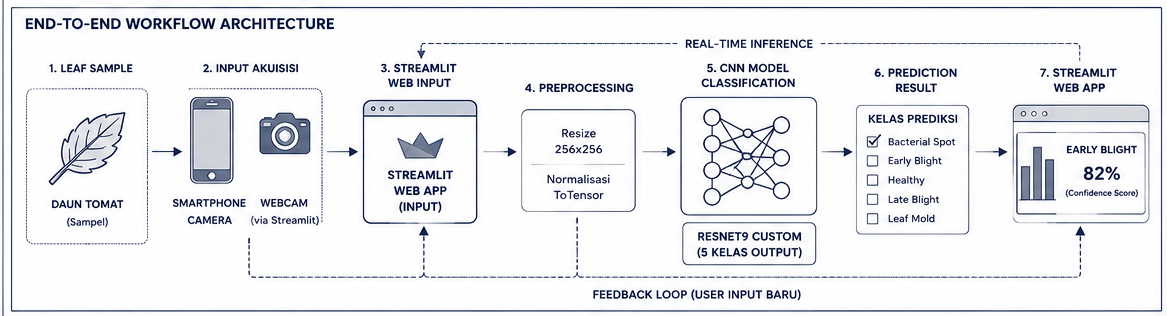
\includegraphics[width=0.9\textwidth]{gambar/end to end.png}
    \caption{Gambaran Alur Kerja (End-to-End Workflow)}
\end{figure}

Sebagaimana diilustrasikan pada Gambar 1.1, alur kerja dalam proyek Machine Learning ini merupakan proses berkesinambungan yang berawal dari pengumpulan dan penyiapan dataset daun tomat, diikuti proses perancangan serta pelatihan model jaringan saraf tiruan. Setelah model dievaluasi dan dianggap memadai, sistem diakhiri dengan proses integrasi (deployment) ke dalam platform aplikasi web interaktif agar model siap digunakan oleh para pengguna akhir.

Sistem ini dirancang tidak untuk memberikan diagnosis final layaknya pandangan pakar agrikultur, melainkan digunakan sebagai alat bantu \textit{screening} awal berdasarkan ciri-ciri visual yang tampak pada gambar daun.

\begin{figure}[htbp]
    \centering
    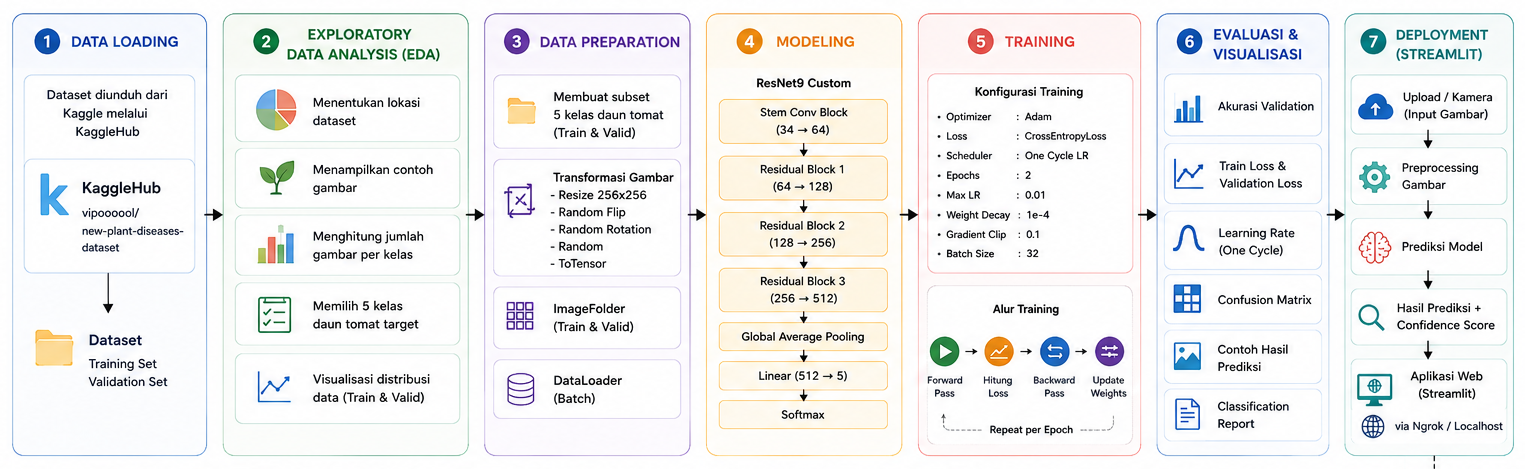
\includegraphics[width=0.85\textwidth]{gambar/pipe line.png}
    \caption{Detail Pipeline Pemrosesan Data dan Pemodelan}
\end{figure}

Lebih rinci lagi, struktur (pipeline) komputasi di bawah kap mesin dapat divisualisasikan pada Gambar 1.2. Alur komputasi ini memperlihatkan transformasi gambar asli ke dalam matriks angka (Tensor) yang sesuai dengan kerangka kerja PyTorch, yang selanjutnya akan diproses secara matematis oleh lapisan-lapisan (layers) pada model arsitektur ResNet9 guna membedakan pola penyakit pada daun tomat.

\section{Tujuan Praktikum}
Adapun tujuan utama dari pelaksanaan praktikum ini adalah sebagai berikut:
\begin{enumerate}
    \item Memberikan pengalaman praktik alur kerja (workflow) pembuatan model Machine Learning secara utuh.
    \item Membuat model Machine Learning untuk mengklasifikasikan gambar daun tomat.
    \item Menampilkan hasil prediksi model dalam bentuk aplikasi web sederhana.
    \item Memahami bahwa model memiliki batasan dan hanya valid untuk data yang sesuai dengan domain pelatihan.
\end{enumerate}

\section{Batasan Sistem}
Untuk memastikan fokus pembelajaran tetap terarah, sistem yang akan dibangun memiliki beberapa batasan:
\begin{itemize}
    \item Dataset difokuskan secara eksklusif pada \textbf{5 kelas kondisi daun tomat}:
    \begin{enumerate}
        \item Bacterial Spot
        \item Early Blight
        \item Late Blight
        \item Leaf Mold
        \item Healthy (Sehat)
    \end{enumerate}
    \item Sistem tidak dapat digunakan untuk memprediksi jenis tanaman lain.
    \item Model yang dilatih belum dilengkapi dengan kelas penolakan (seperti kelas `Unknown` atau `Non Leaf`), sehingga input gambar diasumsikan selalu berupa daun tomat.
\end{itemize}

\section{Persiapan Lingkungan Praktikum}
Pada praktikum ini, spesifikasi komputer lokal yang tinggi tidak diwajibkan karena seluruh proses komputasi, termasuk pelatihan model yang membutuhkan GPU, akan dilakukan di \textit{cloud}. Berikut adalah \textit{tools} dan lingkungan yang perlu dipersiapkan:

Berikut adalah rincian masing-masing teknologi yang menjadi tulang punggung praktikum ini:

\begin{itemize}
    \item \textbf{Google Colab}: Lingkungan Jupyter Notebook gratis berbasis cloud dari Google yang menyediakan akses ke GPU. Digunakan untuk mengeksekusi kode Python, melatih model, dan menjalankan *server* aplikasi.
    \item \textbf{KaggleHub}: Library untuk mengunduh dataset secara langsung dari Kaggle ke environment Google Colab.
    \item \textbf{PyTorch dan Torchvision}: Framework Deep Learning yang akan digunakan untuk mengelola dataset dan membangun arsitektur jaringan saraf tiruan (ResNet9).
    \item \textbf{Streamlit}: Framework open-source berbasis Python untuk membuat antarmuka web interaktif khusus Machine Learning.
    \item \textbf{Ngrok}: Layanan \textit{tunneling} yang memungkinkan aplikasi Streamlit yang berjalan di \textit{localhost} Google Colab dapat diakses melalui internet menggunakan tautan publik.
\end{itemize}

Pastikan Anda telah memiliki akun Google untuk menggunakan Google Colab. Pada bab selanjutnya, kita akan mulai mempersiapkan *environment* praktikum.

\chapter{Persiapan dan Eksplorasi Data}

Bab ini akan memandu Anda dalam mempersiapkan seluruh kebutuhan data yang akan digunakan pada praktikum ini. Terdapat tiga tahapan utama yang akan dilalui, yaitu pengambilan data (\textit{data loading}) dari KaggleHub, persiapan \textit{environment} dengan mengimpor seluruh \textit{library} yang dibutuhkan, serta eksplorasi data awal (\textit{Exploratory Data Analysis} / EDA) untuk memahami karakteristik dataset yang akan digunakan.

\section{Data Loading dengan KaggleHub}

Langkah pertama yang harus dilakukan adalah mengambil dataset gambar daun tanaman dari KaggleHub. Dataset akan digunakan sebagai bahan utama untuk melatih model \textit{Machine Learning} agar mampu mengenali kondisi kesehatan tanaman berdasarkan citra daun.

\subsection{Pengambilan Data}

Tahap awal untuk memulai praktikum ini adalah mendatangkan bahan baku berupa ribuan foto tanaman dari repositori \textit{online} ke dalam lingkungan komputasi kita. Dataset yang digunakan berasal dari Kaggle dengan nama \texttt{vipoooool\allowbreak/new\allowbreak-plant\allowbreak-diseases\allowbreak-dataset}.

KaggleHub adalah \textit{library} Python yang memungkinkan kita mengunduh dataset dari Kaggle secara langsung tanpa perlu mengunduh secara manual melalui \textit{browser}. Dengan menggunakan KaggleHub, dataset akan secara otomatis diunduh dan diekstrak ke dalam \textit{path} yang dapat langsung digunakan.

Berikut adalah kode untuk mengunduh dataset:

\begin{lstlisting}[language=Python, caption=Mengunduh dataset dari KaggleHub]
import kagglehub

# Mengunduh dataset Plant Disease dari KaggleHub
dataset_path = kagglehub.dataset_download(
    "vipoooool/new-plant-diseases-dataset"
)

# Menampilkan lokasi dataset yang berhasil diunduh
print("Dataset berhasil diunduh.")
print("Lokasi dataset:", dataset_path)
\end{lstlisting}

Ketika kode di atas dijalankan, KaggleHub akan mengunduh dataset dan menyimpannya ke dalam direktori \textit{cache} lokal. Variabel \texttt{dataset\_path} akan menyimpan lokasi lengkap dari dataset yang telah diunduh. Lokasi ini nantinya akan digunakan pada tahap-tahap selanjutnya untuk mengakses gambar-gambar yang akan diproses.

Output yang akan tampil setelah kode dijalankan adalah sebagai berikut:

\begin{lstlisting}[language={}, caption=Output pengunduhan dataset]
Dataset berhasil diunduh.
Lokasi dataset: /kaggle/input/new-plant-diseases-dataset
\end{lstlisting}

\begin{tcolorbox}[title=Catatan Penting, colback=blue!5!white, colframe=blue!70!black]
Pastikan Anda telah terhubung ke internet saat menjalankan kode di atas. Dataset yang diunduh memiliki ukuran yang cukup besar, sehingga proses pengunduhan mungkin memerlukan waktu beberapa saat tergantung pada kecepatan koneksi internet Anda.
\end{tcolorbox}

\subsection{Mengecek Struktur Folder Dataset}

Setelah dataset berhasil diunduh, langkah berikutnya adalah mengecek isi folder utama dataset. Tahap ini penting karena setiap dataset Kaggle bisa memiliki struktur folder yang berbeda. Dengan melihat isi folder utama, kita dapat menentukan lokasi folder \texttt{train}, \texttt{valid}, dan \texttt{test} yang akan digunakan pada proses pelatihan model.

Berikut adalah kode untuk mengecek struktur folder dataset:

\begin{lstlisting}[language=Python, caption=Mengecek struktur folder dataset]
import os

# Menampilkan lokasi dataset
print("Lokasi dataset:")
print(dataset_path)

# Mengecek isi folder utama dataset
print("\nIsi folder utama dataset:")

for item in os.listdir(dataset_path):
    item_path = os.path.join(dataset_path, item)

    if os.path.isdir(item_path):
        print(f"[Folder] {item}")
    else:
        print(f"[File] {item}")
\end{lstlisting}

Setelah kode di atas dijalankan, akan terlihat struktur folder dataset sebagai berikut:

\begin{lstlisting}[language={}, caption=Output struktur folder dataset]
Lokasi dataset:
/kaggle/input/new-plant-diseases-dataset

Isi folder utama dataset:
[Folder] New Plant Diseases Dataset(Augmented)
[Folder] new plant diseases dataset(augmented)
[Folder] test
\end{lstlisting}

Dari output tersebut, kita dapat melihat bahwa dataset terdiri dari tiga folder utama. Dua di antaranya merupakan folder yang berisi data \textit{training} dan \textit{validation} yang sudah di-\textit{augmentasi}, serta satu folder \texttt{test} yang berisi data pengujian. Pada praktikum ini, kita akan menggunakan folder yang berisi data \textit{augmented} untuk melatih dan mengevaluasi model.

\section{Persiapan Environment}

Sebelum memulai proses pengolahan data dan pemodelan, kita perlu menyiapkan \textit{environment} dengan mengimpor seluruh \textit{library} yang dibutuhkan. \textit{Library} yang akan digunakan meliputi \textit{library} untuk pengelolaan data, visualisasi, dan \textit{deep learning}.

\subsection{Mengimpor Library}

Berikut adalah kode untuk mengimpor seluruh \textit{library} yang dibutuhkan dalam praktikum ini:

\begin{lstlisting}[language=Python, caption=Mengimpor library yang dibutuhkan]
# Library untuk pengelolaan file dan data
import os
import numpy as np
import pandas as pd

# Library untuk visualisasi
import matplotlib.pyplot as plt
from PIL import Image

# Library utama PyTorch
import torch
import torch.nn as nn
import torch.nn.functional as F

# Library untuk pengolahan dataset dan DataLoader
from torch.utils.data import DataLoader
from torchvision.datasets import ImageFolder
import torchvision.transforms as transforms
from torchvision.utils import make_grid

# Library untuk melihat ringkasan arsitektur model
from torchsummary import summary

# Menampilkan plot langsung di notebook
%matplotlib inline

print("Semua library berhasil diimport.")
\end{lstlisting}

Setelah kode di atas dijalankan, akan muncul output berikut:

\begin{lstlisting}[language={}, caption=Output impor library]
Semua library berhasil diimport.
\end{lstlisting}

Penjelasan masing-masing \textit{library} yang diimpor:

\begin{itemize}
    \item \texttt{os} --- Digunakan untuk mengelola file dan direktori.
    \item \texttt{numpy} --- Library untuk komputasi numerik dan operasi matriks.
    \item \texttt{pandas} --- Library untuk manipulasi dan analisis data tabular.
    \item \texttt{matplotlib.pyplot} --- Library untuk membuat grafik dan visualisasi data.
    \item \texttt{PIL.Image} --- Library untuk membuka dan memproses gambar.
    \item \texttt{torch} --- Library utama PyTorch untuk \textit{deep learning}.
    \item \texttt{torch.nn} --- Modul PyTorch untuk membangun arsitektur jaringan saraf tiruan.
    \item \texttt{torch.nn.functional} --- Modul PyTorch untuk fungsi-fungsi aktivasi dan \textit{loss}.
    \item \texttt{DataLoader} --- Digunakan untuk memuat data dalam bentuk \textit{batch}.
    \item \texttt{ImageFolder} --- Dataset loader khusus untuk data gambar terstruktur dalam folder.
    \item \texttt{transforms} --- Modul untuk melakukan transformasi gambar.
    \item \texttt{make\_grid} --- Utility untuk menampilkan kumpulan gambar dalam bentuk grid.
    \item \texttt{torchsummary} --- Library untuk menampilkan ringkasan arsitektur model.
\end{itemize}

\subsection{Menginstal Library Tambahan}

Beberapa \textit{library} mungkin belum tersedia di \textit{environment} Google Colab secara bawaan. Oleh karena itu, kita perlu menginstalnya terlebih dahulu menggunakan \texttt{pip}. Salah satu \textit{library} yang perlu diinstal adalah \texttt{torchsummary}:

\begin{lstlisting}[language=Python, caption=Menginstal library torchsummary]
!pip install torchsummary -q

print("Library torchsummary berhasil diinstall.")
\end{lstlisting}

Output yang akan tampil:

\begin{lstlisting}[language={}, caption=Output instalasi torchsummary]
Library torchsummary berhasil diinstall.
\end{lstlisting}

\begin{tcolorbox}[title=Catatan Penting, colback=blue!5!white, colframe=blue!70!black]
Perintah \texttt{!pip install} hanya perlu dijalankan satu kali pada awal sesi Google Colab. Jika \textit{runtime} di-reset, Anda perlu menginstal ulang \textit{library} yang tidak termasuk dalam bawaan Colab.
\end{tcolorbox}

Setelah semua \textit{library} berhasil diimpor dan diinstal, \textit{environment} praktikum siap digunakan untuk tahap selanjutnya, yaitu eksplorasi data awal (\textit{Exploratory Data Analysis}).

\section{Exploratory Data Analysis (EDA)}

Setelah dataset berhasil dimuat dan \textit{environment} siap, tahap berikutnya adalah melakukan \textit{Exploratory Data Analysis} (EDA). EDA digunakan untuk memahami kondisi awal dataset, seperti jumlah total gambar, struktur folder, jumlah kelas, dan sebaran data pada setiap kelas. Tahap ini penting agar kita mengetahui apakah dataset sudah layak digunakan untuk proses \textit{training} model \textit{Machine Learning}.

\subsection{Menentukan Lokasi Folder Dataset}

Sebelum melakukan EDA, kita perlu menentukan lokasi folder dataset yang akan digunakan. Pada dataset ini, data \textit{training} dan \textit{validation} berada di dalam folder \texttt{New Plant Diseases Dataset(Augmented)}. Folder \texttt{train} digunakan untuk melatih model, sedangkan folder \texttt{valid} digunakan untuk mengevaluasi performa model selama proses \textit{training}.

Tahap ini penting karena variabel \texttt{train\_dir}, \texttt{valid\_dir}, dan \texttt{diseases} akan digunakan pada proses EDA dan \textit{preprocessing} berikutnya.

Berikut adalah kode untuk menentukan lokasi folder dataset:

\begin{lstlisting}[language=Python, caption=Menentukan lokasi folder dataset]
import os

# Path ke folder dataset utama
dataset_main = os.path.join(
    dataset_path,
    "New Plant Diseases Dataset(Augmented)",
    "New Plant Diseases Dataset(Augmented)"
)

# Path ke folder training dan validation
train_dir = os.path.join(dataset_main, "train")
valid_dir = os.path.join(dataset_main, "valid")

# Menampilkan lokasi folder
print("Folder dataset utama :", dataset_main)
print("Folder training      :", train_dir)
print("Folder validation    :", valid_dir)

# Mendapatkan daftar kelas (nama folder dalam train)
diseases = os.listdir(train_dir)
print("Jumlah kelas dataset :", len(diseases))
\end{lstlisting}

Output yang akan tampil:

\begin{lstlisting}[language={}, caption=Output lokasi folder dataset]
Folder dataset utama : /kaggle/input/new-plant-diseases-dataset/New Plant
                        Diseases Dataset(Augmented)/New Plant Diseases
                        Dataset(Augmented)
Folder training      : /kaggle/input/new-plant-diseases-dataset/New Plant
                        Diseases Dataset(Augmented)/New Plant Diseases
                        Dataset(Augmented)/train
Folder validation    : /kaggle/input/new-plant-diseases-dataset/New Plant
                        Diseases Dataset(Augmented)/New Plant Diseases
                        Dataset(Augmented)/valid
Jumlah kelas dataset : 38
\end{lstlisting}

Dari output di atas, kita dapat melihat bahwa dataset utama memiliki total 38 kelas penyakit tanaman. Namun, untuk praktikum ini kita hanya akan fokus pada 5 kelas daun tomat.

\subsection{Menghitung Total Gambar dalam Dataset}

Setelah mengetahui struktur folder, langkah selanjutnya adalah menghitung total seluruh gambar yang tersedia untuk memastikan kita memiliki cukup banyak contoh foto untuk dipelajari oleh model.

Berikut adalah kode untuk menghitung total gambar dalam dataset:

\begin{lstlisting}[language=Python, caption=Menghitung total gambar dalam dataset]
# Ekstensi file gambar yang akan dihitung
image_extensions = (".jpg", ".jpeg", ".png")

# Variabel untuk menyimpan jumlah total gambar
total_images = 0

# Menelusuri seluruh folder dan subfolder dataset
for root, dirs, files in os.walk(dataset_path):
    image_files = [
        file for file in files
        if file.lower().endswith(image_extensions)
    ]

    total_images += len(image_files)

# Menampilkan hasil
print("Total gambar dalam dataset:", total_images)
\end{lstlisting}

Setelah kode dijalankan, akan tampil output berikut:

\begin{lstlisting}[language={}, caption=Output total gambar dalam dataset]
Total gambar dalam dataset: 175767
\end{lstlisting}

Kode di atas akan menelusuri seluruh folder dan subfolder dalam dataset, kemudian menghitung jumlah file gambar dengan ekstensi \texttt{.jpg}, \texttt{.jpeg}, dan \texttt{.png}. Hasilnya menampilkan total seluruh gambar yang tersedia di dalam dataset, yaitu sebanyak \textbf{175.767} gambar.

\subsection{Menampilkan Contoh Gambar Dataset}

Setelah mengetahui jumlah total gambar, langkah selanjutnya adalah melihat contoh gambar dari dataset. Hal ini penting untuk memahami karakteristik visual dari data yang akan diproses, seperti ukuran gambar, kualitas resolusi, dan variasi kondisi daun yang ada.

Berikut adalah kode untuk menampilkan contoh gambar dari dataset:

\begin{lstlisting}[language=Python, caption=Menampilkan contoh gambar dataset]
# Ekstensi gambar yang akan dicari
image_extensions = (".jpg", ".jpeg", ".png")

# Menyimpan seluruh path gambar
image_paths = []

# Menelusuri seluruh folder dataset
for root, dirs, files in os.walk(dataset_path):
    for file in files:
        if file.lower().endswith(image_extensions):
            image_paths.append(os.path.join(root, file))

# Menampilkan jumlah gambar yang ditemukan
print("Jumlah gambar ditemukan:", len(image_paths))

# Mengecek apakah ada gambar yang ditemukan
if len(image_paths) == 0:
    print("Tidak ada gambar yang ditemukan. Periksa kembali lokasi dataset.")
else:
    # Mengambil gambar pertama sebagai contoh
    sample_image_path = image_paths[0]

    # Membuka gambar
    img = Image.open(sample_image_path).convert("RGB")

    # Menampilkan informasi gambar
    print("Contoh path gambar:")
    print(sample_image_path)
    print("Ukuran gambar:", img.size)

    # Menampilkan gambar
    plt.figure(figsize=(5, 5))
    plt.imshow(img)
    plt.axis("off")
    plt.title("Contoh Gambar Dataset")
    plt.show()
\end{lstlisting}

Output yang akan tampil setelah kode dijalankan:

\begin{lstlisting}[language={}, caption=Output teks contoh gambar dataset]
Jumlah gambar ditemukan: 175767
Contoh path gambar:
/kaggle/input/new-plant-diseases-dataset/New Plant
Diseases Dataset(Augmented)/New Plant Diseases
Dataset(Augmented)/valid/Tomato___Late_blight/1e5ba644-
efeb-4bd3-b878-a0606cf8a992___RS_Late.B 6272_flipLR.JPG
Ukuran gambar: (256, 256)
\end{lstlisting}

Selain informasi di atas, kode tersebut juga akan menampilkan visualisasi gambar secara langsung. Gambar \ref{fig:contoh_dataset} berikut adalah contoh gambar yang dihasilkan:

\begin{figure}[H]
\centering
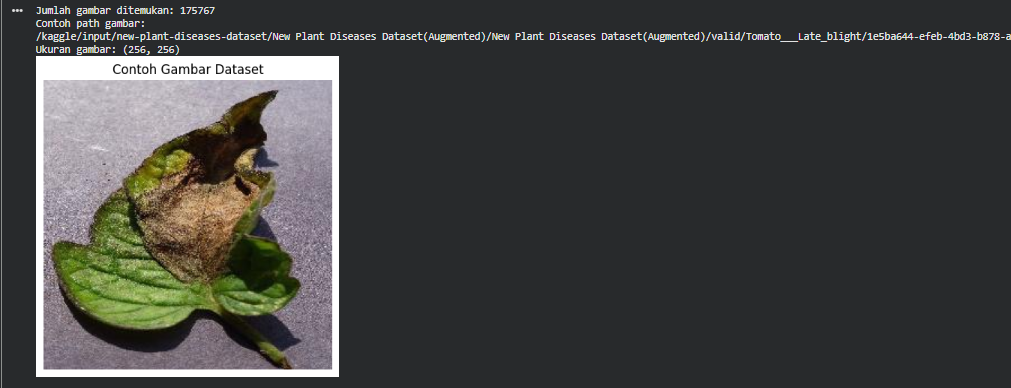
\includegraphics[width=0.6\textwidth]{gambar/2.3.png}
\caption{Contoh gambar daun dari dataset}
\label{fig:contoh_dataset}
\end{figure}

Dari output di atas, kita dapat melihat bahwa setiap gambar dalam dataset memiliki ukuran \textbf{256\texttimes256} piksel. Gambar contoh yang ditampilkan berasal dari kelas \texttt{Tomato\_\_\_Late\_blight} (penyakit hawar daun tomat). Selain informasi path dan ukuran, kode di atas juga akan menampilkan visualisasi gambar secara langsung di \textit{notebook}.

\begin{tcolorbox}[title=Catatan Penting, colback=blue!5!white, colframe=blue!70!black]
Pada lingkungan Google Colab, perintah \texttt{plt.show()} akan menampilkan gambar langsung di bawah sel kode. Jika Anda menjalankan kode di \textit{terminal} biasa, pastikan \textit{backend} matplotlib telah dikonfigurasi dengan benar untuk menampilkan grafik.
\end{tcolorbox}


\end{document}
